\section{la citadelle}

\includegraphics[width=200pt]{_img/places/citadel-of-ktath-atn.png}

\textbf{Ktath’Atn} est une planète peu accueillante, il y pleut presque tout le temps. L’Empire n’y a aucune prise, la reine y règne d’une main de fer, sans pitié ni compassion. Il lui arrive d’être magnanime mais jamais sans raison. La \nameref{sec:ktath-atn-queen} est imprévisible et il ne faut pas la sous-estimer, sous ses aspects gracieux se cache une tigresse sans pitié.

\begin{paperbox}{Séquence Narrative}
Ici commence une section narrative, sans combat (normalement). À vous de mettre les joueurs dans l’ambiance, il sera possible d’utiliser des compétences de charisme et de persuasion. Cette séquence est longue à écrire et à lire mais ne devrait pas durer des heures à jouer.
\end{paperbox}

\subsection{L’accueil}

\begin{wrapfigure}{r}{0.3\linewidth}
    \vspace{-4\baselineskip}
    \centering\hspace*{-.99\columnsep}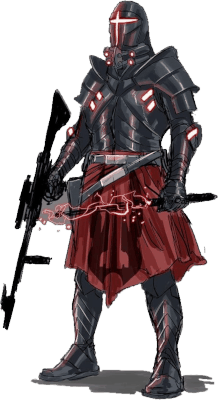
\includegraphics[width=1.2\linewidth]{_img/bestiary/citadel-guard.png}
    \vspace{-1\baselineskip} 
\end{wrapfigure}

\'A leur arrivée dans le périmètre de Ktath’Atn, les héros et leur vaisseau sont dirigés vers une plateforme d’atterrissage où ils sont attendu par 4 \nameref{sec:citadel-guard} pour être escorté vers leurs quartiers avant la réception de ce soir.

L’un des gardes demande l’invitation, \nameref{sec:aphra} lui tend le document et les gardes font signe de les suivre. Ils encadrent le groupe ne laissant que peu de marge de manœuvre aux héros.

Les quartiers des invités se situent dans les premiers étages de la tour. Ce sont des appartements luxueux avec largement assez de place pour que chaque membre du groupe est de quoi poser ses affaires.

Le soir tombe sur la citadelle. Laissez les héros faire ce qu’ils souhaitent pour se préparer à la réception. Les blasters et les lames ne seront pas autorisés durant la soirée, une tenue correcte est de rigueur sous peine de perdre \textbf{-2 Cha}risme. 

\subsection{La réception}

Les héros débarquent dans une salle immense, style cathédrale, très haut de plafond, colonnes, \dots

\'A l’intérieur une centaine de personnes, de toutes espèces et de tous genres. Certains humanoïdes, d’autres d’aspect gélatineux, mais tous organiques. Des droïdes font le service au milieu des invités. 

Si un ou plusieurs de vos héros sont des droïdes, ils ne se sentent pas à l’aise, ils perdent \textbf{-1 Cha}risme durant la soirée.

\begin{paperbox}{Mission bonus}
Plusieurs types d’interactions sont possibles durant cette phase de la soirée. Un jet de \textbf{Pers}uasion \textbf{Diff}iculté \textbf{6} incitera les convives à parler à vos héros. Deux types d’informations sont alors disponibles, au MJ de distiller les infos selon ses préférences.

Les héros peuvent tenter d’en apprendre plus sur \nameref{sec:aphra}. S’ils posent la question aux bonnes personnes et que le jet est réussi, ils apprendront que \nameref{sec:aphra} n’est pas très fiable. Une partie des convives s’est déjà fait arnaqué par \nameref{sec:aphra} et serait ravi de lui rendre la pareille. Elle est clairement dans le commerce de droïdes de combat et en sait forcément plus que ce qu’elle a dit aux héros jusque-là.

Les héros peuvent aussi apprendre ce que les autres invités ont prévu de présenter à la reine pour obtenir ses faveurs. Dans le tas, une sorte de fée clochette capable de répandre une poudre qui permet aux humanoïdes de voler pendant une courte durée. Un guerrier Ezarien muni d’un exosquelette naturel. Une sorte de taupe, capable de se téléporter sur courte distance quand elle éternue, \dots

Au MJ d’échanger avec les joueurs sachant que de toutes façons, la reine choisira vos héros comme vainqueurs.

Ce passage n’est pas obligatoire, si vos joueurs sont plus portés sur la castagne, ou si vous n’êtes pas un MJ aguerri à l’improvisation, ne vous lancez pas là-dedans.
\end{paperbox}

Quand le MJ décide qu’il est temps (les joueurs n’intérragissent pas/plus) c’est le moment de faire entrer la reine et ses sbires.\\

\noindent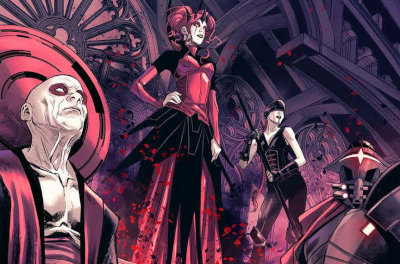
\includegraphics[width=\linewidth]{_img/places/queen-with-minions.jpg}

\begin{quotebox}
Bonsoir et merci à vous mes chers amis d’être venu ce soir, il me tarde de voir ce que vous avez à me présenter. Et comme promis celui qui me présentera la forme de vie organique la plus “intéressante” se verra accorder une de mes faveurs.

Mais ne traînons plus, commençons les présentations immédiatement.
\end{quotebox}

\nameref{sec:varroa} prend alors la parole et commence à appeler les invités un à un.

\begin{paperbox}{Présentations}
Je ne décris pas ici chaque présentation qui est faite. Je laisse au MJ le soin et l’imagination de faire passer des êtres plus ou moins étranges qui seront dignes ou non d’intérêt. Quand les joueurs ont compris le principe, c’est à eux d’entrer en scène.
\end{paperbox}

\begin{quotebox}
\noindent\textbf{\nameref{sec:varroa}}: Docteur Aphra

\emph{\nameref{sec:aphra} fait signe aux héros de s’avancer avec elle.}

\noindent\textbf{\nameref{sec:varroa}}: Qu’avez-vous à présenter à la reine.\\
\noindent\textbf{\nameref{sec:aphra}}: Un Jedi humain

\emph{Ou n’importe quoi selon les héros que vous avez.}
\end{quotebox}

\'A ces mots un, silence assourdissant se fit entendre. Un guerrier Ezarien sort de la foule et prend \nameref{sec:aphra} à partie. Il est grand, fin et possède une sorte d’exosquelette qui le protège des coups directs.

\begin{quotebox}
C’est une blague, les Jedis ont été éradiqués, qu’est-ce que cet humain va pouvoir faire contre moi !
\end{quotebox}

Et le guerrier Ezarien se jette sur le Jedi. Vu que ce dernier a clairement montré ses intentions, la première attaque est pour le Jedi. L’enjeu ici est de faire une démonstration des pouvoirs à la reine. \'A la première utilisation visible des pouvoirs de Jedi, \nameref{sec:varroa} stoppe le combat. De son côté, le guerrier Ezarien n’a que ses poings.

Si par hasard le Jedi n’a pas accès à des pouvoirs visibles, laissez-le se prendre quelques coups puis faites lui utiliser une \textbf{Poussée de Force} instinctive contre le guerrier. Cela suffira à impressionner la reine qui mettra fin au combat.

\begin{quotebox}
\noindent\textbf{\nameref{sec:varroa}}: La reine a choisi, tous les invités doivent partir immédiatement, la réception est terminée.

\emph{\nameref{sec:varroa} fait signe aux héros de s’avancer vers lui.}

\noindent\textbf{\nameref{sec:varroa}}: Ce soir nous vous offrons l’hospitalité. Demain vous déjeunerez avec la Reine, elle écoutera votre requête à ce moment. Allez dormir maintenant.
\end{quotebox}

Vos héros ont déjà pas mal bougé, ils vont se coucher. Pas d’exploration pour l’instant, on verra demain.
